\documentclass[a4paper]{article}
\usepackage[utf8]{inputenc}
\usepackage[spanish, es-tabla]{babel}
\usepackage[margin=0.7in]{geometry}
\usepackage{amsmath}
\usepackage{amsfonts}
\usepackage{amssymb}
\usepackage{xcolor}

\usepackage{float}
\usepackage{graphicx}
\graphicspath{ {./Imagenes/} }

\usepackage[american voltages,american currents]{circuitikz}

\usepackage{fancyhdr}

\usepackage{units} 

\pagestyle{fancy}
\fancyhf{}
%\lhead{23.09 Física Electrónica}
\rhead{Bertachini, Lambertucci, Londero, Mechoulam, Musich}
\rfoot{Página \thepage}


\begin{document}

%%%%%%%%%%%%%%%%%%%%%%%%%%%%%%%%%%%%%%%%%%%%%%%%%%%%%%%%%%%%%%%%%%%%%%%%% 
%								CARATULA								%
%%%%%%%%%%%%%%%%%%%%%%%%%%%%%%%%%%%%%%%%%%%%%%%%%%%%%%%%%%%%%%%%%%%%%%%%% 

\begin{titlepage}
\newcommand{\HRule}{\rule{\linewidth}{0.5mm}}
\center
\mbox{\textsc{\LARGE \bfseries {Instituto Tecnológico de Buenos Aires}}}\\[1.5cm]
\textsc{\Large 23.09 Física Electrónica}\\[0.5cm]

\HRule \\[0.6cm]
{ \Huge \bfseries Trabajo práctico N$^{\circ}$1}\\[0.4cm] 
\HRule \\[1.5cm]


{\large

\emph{Grupo 5}\\
\vspace{3px}

\begin{tabular}{lr}
\textsc{Bertachini}, Germán  & 58750 \\ 	
\textsc{Lambertucci}, Guido Erinque  & 58009 \\
\textsc{Londero Bonaparte}, Tomás Guillermo  & 58150 \\
\textsc{Mechoulam}, Alan  &  58438\\
\textsc{Musich}, Francisco  & 58124 \\

\end{tabular}

\vspace{20px}

\emph{Profesores}\\
\vspace{3px}
\textsc{Baez}, Eduardo Diocles\\ 	
\textsc{Cesaretti}, Juan Manuel\\ 
\textsc{Douthat}, Analia Elizabeth\\ 
\textsc{Gardella}, Pablo Jesús\\ 	

\vspace{100px}

\begin{tabular}{ll}

Presentado: & 24/06/19\\

\end{tabular}

}

\vfill

\end{titlepage}


%%%%%%%%%%%%%%%%%%%%%%%%%%%%%%%%%%%%%%%%%%%%%%%%%%%%%%%%%%%%%%%%%%%%%%%%% 
%								INFORME									%
%%%%%%%%%%%%%%%%%%%%%%%%%%%%%%%%%%%%%%%%%%%%%%%%%%%%%%%%%%%%%%%%%%%%%%%%%

\section*{Introducción}

En el trabajo presente se llevó adelante el estudio de distintos tipos de diodos y circuitos, con el objetivo de llevar a la práctica la teoría estudiada en clase y contrastar los datos obtenidos con los modelos teóricos.

\section*{Desarrollo de la Experiencia}

\subsection*{Medición de Diodos}

Se realizó la medición de las curvas características de tres diodos distintos: Rectificador 1N4007, Diodo Zener 12 V y LED rojo de 5 mm en ese orden respectivamente. Los diodos fueron conectados de la forma presentada en el circuito (\ref{circ:1}).

\begin{figure}[H]
\begin{center}
\begin{circuitikz}
\draw
	(4,0)	to (0,0)
	(0,1.5)	to [sV,v_=$V$]	(0,0)
	(0,1.5)	to [R, l_=$ 470 \ \Omega $]	(4,1.5)
	(4,0)	to [Do, l_=Diodo analizado]	(4,1.5)
;\end{circuitikz}
\end{center}
\caption{Circuito utilizado para medir los diodos.}
\label{circ:1}
\end{figure}

Haciendo uso de multímetros para el diodo rectificador y el diodo zener, y el osciloscopio para el LED, se observaron los comportamientos de cada diodo a ciertas tensiones para posteriormente graficar las curvas características correspondiente a cada uno.

Se realizó una superposición de las curvas de valores medidos en el laboratorio con las curvas simuladas en \texttt{ltspice} para cada dispositivo.

\begin{figure}[H]
	\centering
	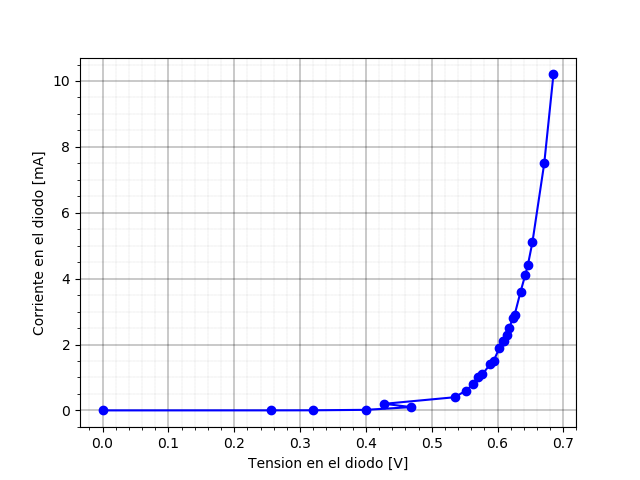
\includegraphics[width=0.7\textwidth]{CurvaDiodoRectificador.png}
	\caption{Superposición de las curva característica medida/simulada del diodo rectificador 1N4148.}
	\label{fig:diodorect}
\end{figure}

\begin{figure}[H]
	\centering
	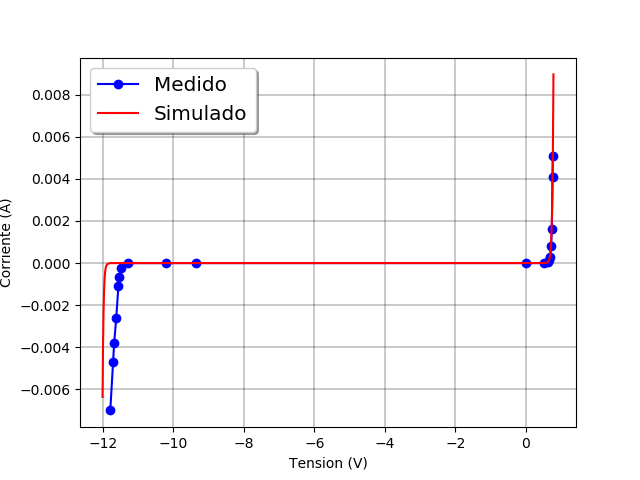
\includegraphics[width=0.7\textwidth]{CurvaZenerEntera.png}
	\caption{Superposición de las curva característica medida/simulada del diodo zener.}
	\label{fig:diodozen}
\end{figure}

Se puede observar que tanto para el diodo rectificador como para el diodo zener las simulaciones realizadas coinciden en su gran mayoría con las mediciones de laboratorio. La mayor discrepancia se encuentra en la tensión de zener $V_Z$, ya que en las simulaciones se puede observar claramente que $V_Z=12 \ V$ en módulo, mientras que las mediciones en el laboratorio sugieren que $V_Z \approx 11,5 \ V$ en módulo.

\begin{figure}[H]
	\centering
	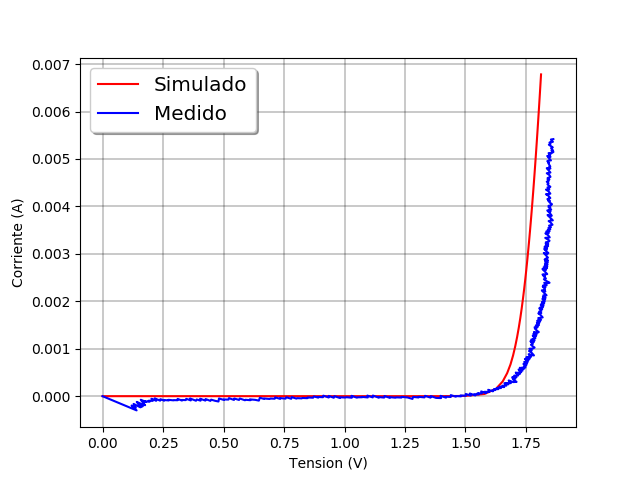
\includegraphics[width=0.7\textwidth]{CurvaDiodosLed.png}
	\caption{Superposición de las curva característica medida/simulada del diodo LED.}
	\label{fig:diodoled}
\end{figure}

Para realizar las mediciones en el diodo LED se optó por el uso del osciloscopio. Se utilizaron dos canales, uno para medir la caída de potencial sobre el diodo y otro para medir la tensión suministrada por la fuente (rampa de 0 V a 5 V). Además, como los diodos poseen un comportamiento capacitivo, se decidió usar las puntas del osciloscopio en x10. Luego, se le restó a esta última la diferencia de potencial en el diodo para obtener la caída sobre la resistencia. Dividiendo por el valor de la resistencia se logró obtener la curva de la corriente. Dada la dispersión de las señales atribuidas al ruido electromagnético captado por el osciloscopio, razón por la cual la curva no se observa suave, se decidió utilizar un suavizamiento exponencial para reducir esta. Finalmente, se graficó de manera superpuesta a la curva de la simulación la curva de la corriente en función de la tensión.
Se puede observar que existen leves discrepancias entre la curva de la simulación y la medición de laboratorio. La mayor diferencia se encuentra en la tensión de foward del LED,en  la cual la discrepancia es de $\approx 0,2 \ V$.
Como el LED utilizado para simulación no fue exactamente el utilizado en el laboratorio, sino fue elegido a causa de las similares características, se consideran aceptables las diferencias entre ambas curvas.

Luego, se puede afirmar que los resultados obtenidos al estudiar los tres primeros diodos se corresponden con los resultados esperados, conclusión a la que se llega al comparar las curvas medidas con las teóricas simuladas en las figuras (\ref{fig:diodozen}), (\ref{fig:diodorect}) y (\ref{fig:diodoled}).

\subsection*{Simulación de Circuito con Transistor}

Se procedió a realizar la simulación del siguiente circuito en \texttt{ltspice} el cual es un amplificador mediante el uso de un transistor npn BC547B:
\begin{figure}[H]
	\centering
	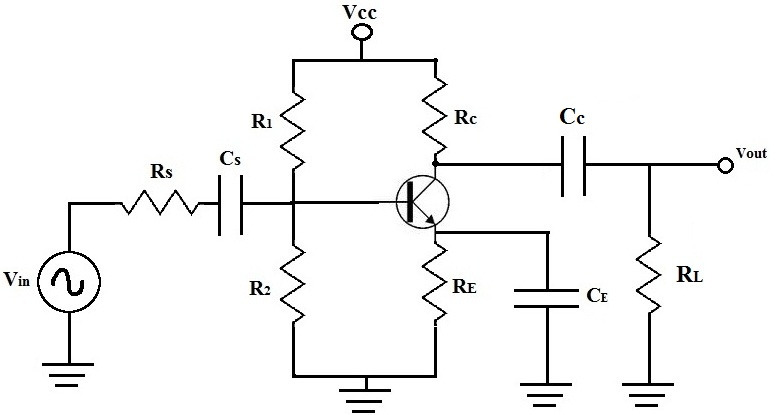
\includegraphics[width=0.6 \textwidth]{commonEmitter.jpg}	
	\caption{Circuito provisto por la cátedra.}
	\label{fig:cmnemitnpn}

\end{figure}

Para este circuito se realizo el análisis de pequeña señal, reduciéndolo al siguiente circuito
\begin{figure}[H]
	\centering
	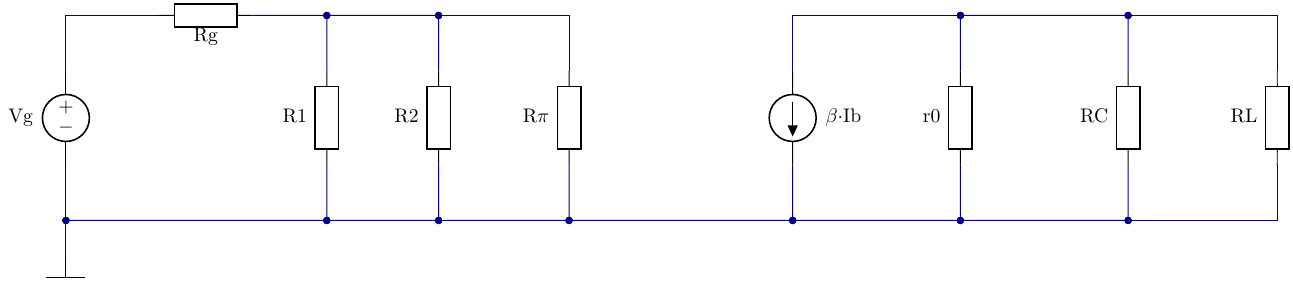
\includegraphics[width=1 \textwidth]{CircEq.PNG}	
	\caption{Analisis de pequeña señal.}
	\label{fig:littleSignal}
\end{figure}

A partir de este modelo se pudo calcular la transferencia en la zona de las frecuencias medias, quedando esta de la siguiente manera: \[H(s)=\frac{R_1\parallel R_2\parallel R_\pi}{R_g+R_1\parallel R_2\parallel R_\pi}\cdot \frac{1}{R_\pi} \cdot \beta \cdot r_0 \parallel R_c \parallel R_L  \]

Se obtuvieron los valores de $R_\pi = 6,32 \cdot 10^{3} \ \Omega$ a partir de la formula \[R_\pi = \frac{V_T}{I_c}\cdot (\beta +1) \] utilizando Ic del spice y calculando $V_T$ $\approx 25 \ mV$ (temperatura ambiente).
El valor de $R_0$ se obtuvo de la simulación, mientras que el de $\beta$, de la datasheet. Como el fabricante da un rango de valores, elegimos un valor de 295.
Valiendose del uso de simulaciones en \texttt{ltspice}, las cuales fueron redibujadas en \texttt{python}, se analiza la función transferencia de tensión del circuito y se observa que para la zona constante, el valor calculado es de $43.82 \ dB$, siendo de $43,19 \ dB$ el valor obtenido en la simulación.

\begin{figure}[H]
	\centering
	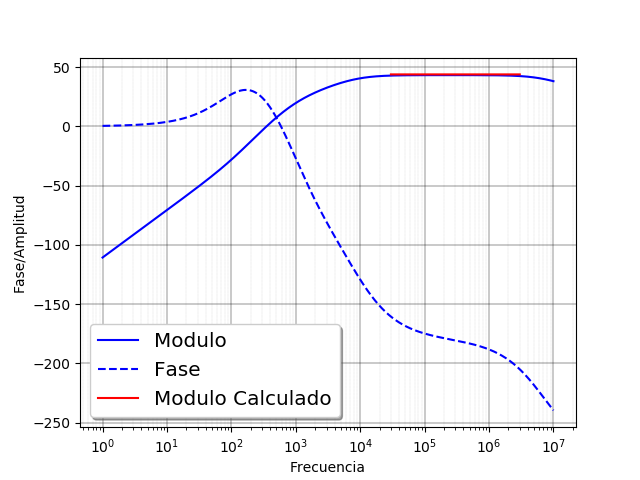
\includegraphics[width=0.9\textwidth]{RtaF2.png}	
	\caption{Diagrama de BODE teórico para el circuito dado, siendo la curva de mayor trazo el diagrama de amplitud.}
	\label{fig:bode}
\end{figure}


\subsection*{Simulación del Circuito con Diodo}

Se quiso analizar la respuesta en frecuencia del circuito en la figura (\ref{circ:3}). Dado que el circuito no posee un comportamiento lineal, se calculó la respuesta de este en su punto de polarización Q utilizando el modelo de pequeña señal. Esto nos permite aproximar su comportamiento a uno lineal.
\begin{figure}[H]
\begin{center}
\begin{circuitikz}[scale=1.5]
\draw

	(0,0)	to (4,0)
	(0,1.5)	to [sV,v_=$AC$]	(0,0)
	(0,2.5)	to [V,v_=$DC$]	(0,1.5)
	(0,2.5)	to[R,l=$R_G$,a=$50\Omega$] (2,2.5)
	(0,2.5)	to[R,l=$R_G$] (2,2.5)
	(2,2.5)	to[R,l=$R$,a=$100K\Omega$] 	(4,2.5)
	(2,2.5)	to[R,l=$R$] 	(4,2.5)
	(4,0)	to [Do, l_=D1N4007]	(4,2.5)
;\end{circuitikz}
\end{center}
\caption{Respuesta en frecuencia del 1N4007.}
\label{circ:3}
\end{figure}

De esta manera, utilizando \texttt{ltsipce}, se obtuvo el diagrama de Bode ilustrado en la figura (\ref{fig:rtaf}).

Se puede observar como el comportamiento de la respuesta en frecuencia es similar a la de un filtro pasabajos de primer orden compuesto por un polo en $f=f_c$. Esto indica que el diodo puede ser asociado a un elemento capacitivo.
Para obtener la frecuencia de corte, se toma el valor de la frecuencia cuando la ganancia es de -3dB, obteniendo \[f_c = f \vert_{|H(f)|= -3 \ dB} \approx 800 \ KHz\].

Para caracterizar al diodo por su circuito equivalente, se utilizó un capacitor en paralelo con una resistencia, debido a que tiene un comportamiento similar a un filtro pasabajos RC. El valor de la resistencia fue obtenida por medio de la simulación la cual es de $1 \ T\Omega$, mientras que la capacitancia del circuito equivalente puede ser calculada como \[c=\frac{1}{2\pi R f_c}\] obteniendo un valor de $1,989 \ pF$. Este valor es similar al obtenido mediante el uso de \texttt{ltspice}, $1,95 \ pF$ respectivamente. Ambos valores se encuentran en el orden de la capacitancia declarada por el fabricante de $4 \ pF$.

Finalmente, la figura (\ref{circ:4}) muestra el circuito equivalente del diodo 1N4007.

\begin{figure}[H]
\begin{center}\begin{circuitikz}[scale=1.8]\draw
(0,1) to[V, l=$DC$,a=$5V$] (0,2)
(0,0) to[sV, l=$AC$,a=$1V$] (0,1)
(0,2) to[R,l=$R_G$]  (2,2)
(2,2) to[R,l=$100K\Omega$] (3,2)
(3,2) -- (5,2)
(3.5,2) to[R,l=$R_D$,a=$1T\Omega$] (3.5,0)
(5,0)	to [C, l=$C$,a=1.95pF]	(5,2)
(0,0) -- (5,0);
\end{circuitikz} 
\end{center}
\caption{Circuito equivalente del diodo.}
\label{circ:4}
\end{figure}

Además, se simuló el diagrama de Bode en \texttt{ltspice} de dicho circuito, curva ilustrada en la figura (\ref{fig:rcmodel}), respaldando el modelo RC utilizado previamente.

\begin{figure}[H]
	\centering
	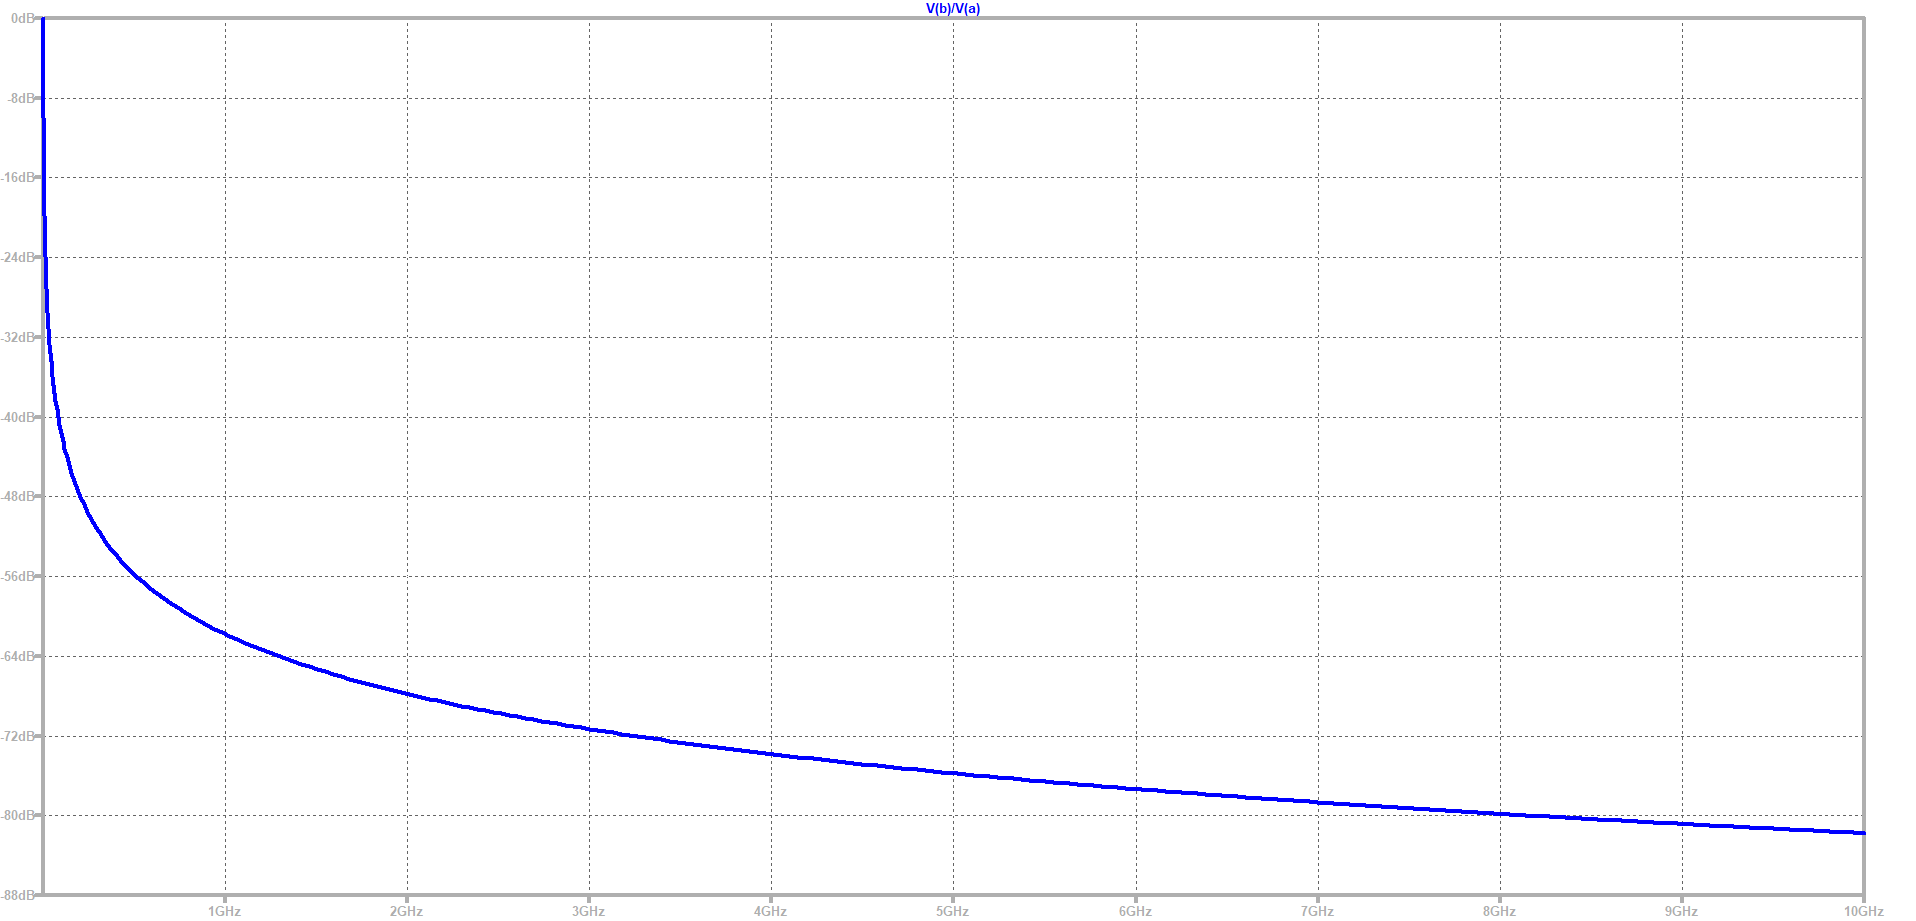
\includegraphics[width=0.9\textwidth]{RtaF3.png}	
	\caption{Respuesta en frecuencia del diodo D1N4007 siendo la curva de mayor trazo el diagrama de amplitud.}
	\label{fig:rtaf}
\end{figure}

\begin{figure}[H]
	\centering
	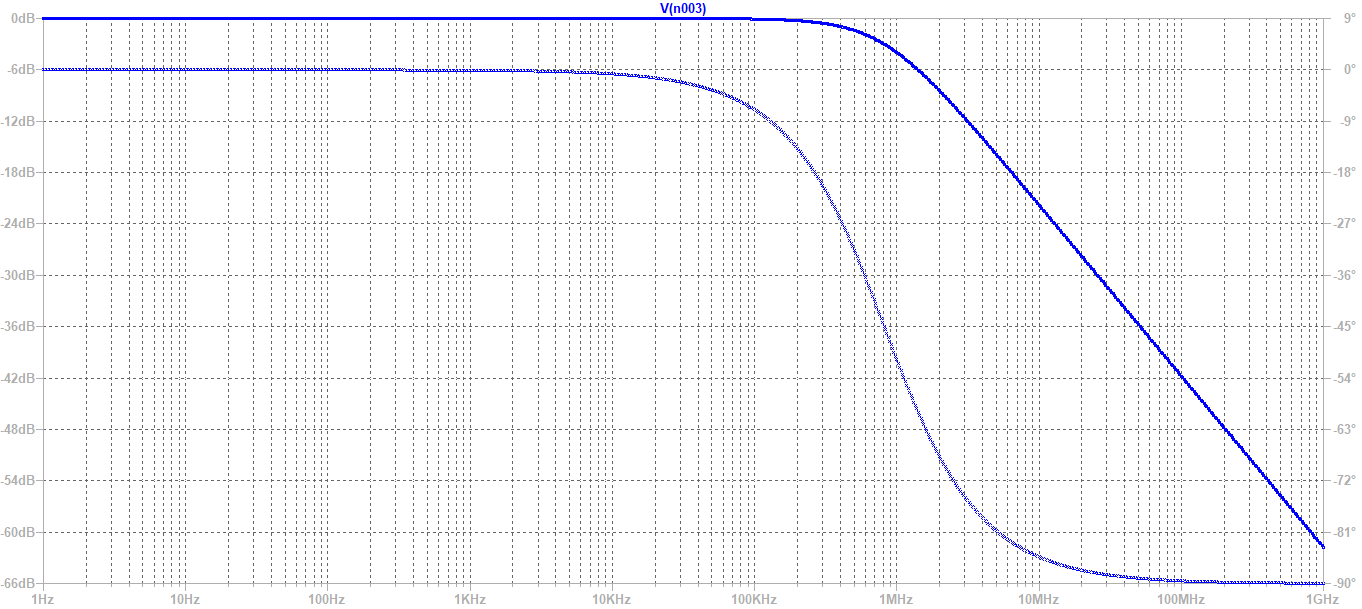
\includegraphics[width=1 \textwidth]{RtaF3RC.png}	
	\caption{Bode del modelo equivalente RC del diodo. La curva solida indica el modulo mientras que la difusa la fase.}
	\label{fig:rcmodel}
\end{figure}



\textcolor{red}{COMPARAR CON MODELO TEORICO!!}\\
\textcolor{red}{NO REPETIR MEDICIONES ES INADMISIBLE}\\
\textcolor{red}{NO EXPLICADO COMO SACAMOS LA GANANCIA}\\
\textcolor{red}{QUE MODELO DE TRANSISTOR USAMOS? COMO SACAMOS RPI R0 GM?? CONSIDERAMOS CAP PARASITA?? PUNTO Q?}\\
\textcolor{red}{REEMPLAZAR DIODO SOLO POR UN CAP ESTA MAL.}\\


\end{document}

